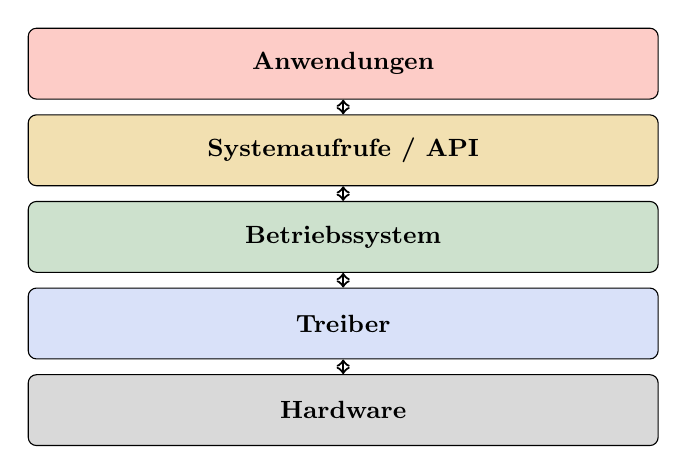
\begin{tikzpicture}[
    layer/.style={draw, minimum width=8cm, minimum height=0.9cm, text centered, rounded corners=3pt, font=\small},
]
    \node[layer, fill=Salmon!40]        (app)  at (0, 3.0) {\textbf{Anwendungen}};
    \node[layer, fill=Goldenrod!35]     (api)  at (0, 1.9) {\textbf{Systemaufrufe / API}};
    \node[layer, fill=DarkSeaGreen!45]  (os)   at (0, 0.8) {\textbf{Betriebssystem}};
    \node[layer, fill=RoyalBlue!20]     (drv)  at (0,-0.3) {\textbf{Treiber}};
    \node[layer, fill=Gray!30]          (hw)   at (0,-1.4) {\textbf{Hardware}};

    \draw[<->, thick] (app) -- (api);
    \draw[<->, thick] (api) -- (os);
    \draw[<->, thick] (os)  -- (drv);
    \draw[<->, thick] (drv) -- (hw);
\end{tikzpicture}
